\documentclass{standalone}
\usepackage{tikz}
\begin{document}
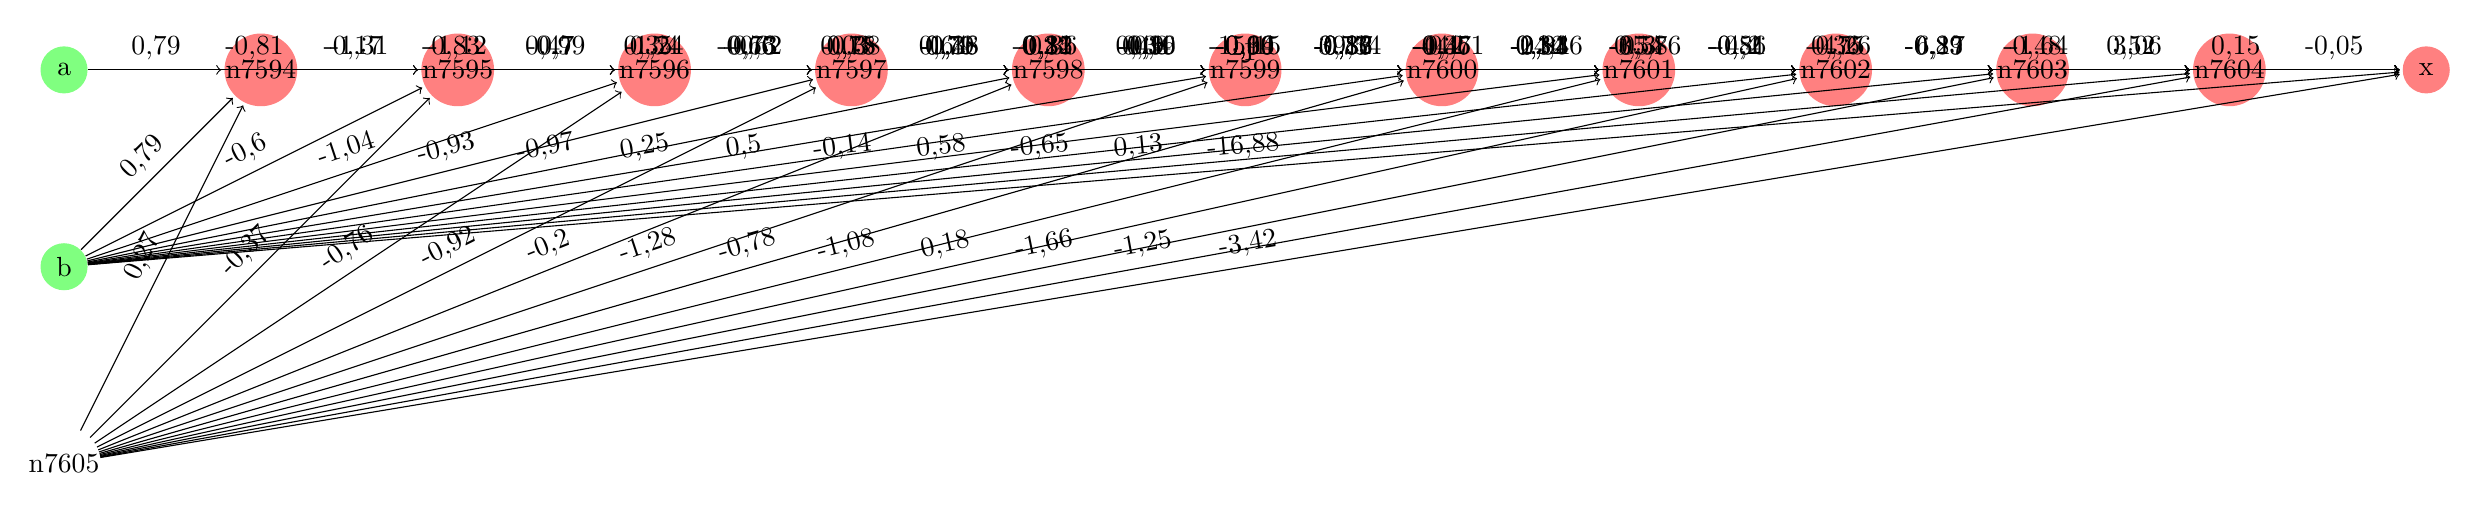
\begin{tikzpicture}[shorten >=1pt,->,draw=black!,node distance=2.5cm]
\tikzstyle{neuron}=[circle,fill=black!25,minimum size=17pt,inner sep=0pt]
\tikzstyle{constant}=[neuron, fill=white!50];
\tikzstyle{sigmoid}=[neuron, fill=red!50];
\tikzstyle{identity}=[neuron, fill=green!50];
\node [identity] (a) {a};
\node [identity,below of=a] (b) {b};
\node [constant,below of=b] (n7605) {n7605};
\node [sigmoid,right of=a] (n7594) {n7594};
\node [sigmoid,right of=n7594] (n7595) {n7595};
\node [sigmoid,right of=n7595] (n7596) {n7596};
\node [sigmoid,right of=n7596] (n7597) {n7597};
\node [sigmoid,right of=n7597] (n7598) {n7598};
\node [sigmoid,right of=n7598] (n7599) {n7599};
\node [sigmoid,right of=n7599] (n7600) {n7600};
\node [sigmoid,right of=n7600] (n7601) {n7601};
\node [sigmoid,right of=n7601] (n7602) {n7602};
\node [sigmoid,right of=n7602] (n7603) {n7603};
\node [sigmoid,right of=n7603] (n7604) {n7604};
\node [sigmoid,right of=n7604] (x) {x};
\path[every node/.style={sloped,anchor=south,auto=false}]
(n7594) edge node {39,54} (x)
(n7594) edge node {-1,31} (n7595)
(n7594) edge node {-1} (n7604)
(n7594) edge node {-1,38} (n7601)
(n7594) edge node {-0,38} (n7600)
(n7594) edge node {0,34} (n7603)
(n7594) edge node {-0,36} (n7602)
(n7594) edge node {-0,99} (n7597)
(n7594) edge node {-1,12} (n7596)
(n7594) edge node {-0,6} (n7599)
(n7594) edge node {-1,24} (n7598)
(n7595) edge node {-44,51} (x)
(n7595) edge node {0,7} (n7596)
(n7595) edge node {-0,36} (n7602)
(n7595) edge node {0,81} (n7601)
(n7595) edge node {-0,82} (n7604)
(n7595) edge node {-0,96} (n7603)
(n7595) edge node {-0,62} (n7598)
(n7595) edge node {0,54} (n7597)
(n7595) edge node {-0,16} (n7600)
(n7595) edge node {0,15} (n7599)
(n7596) edge node {0,73} (n7597)
(n7596) edge node {-24,36} (x)
(n7596) edge node {0,73} (n7603)
(n7596) edge node {-0,39} (n7602)
(n7596) edge node {0,4} (n7604)
(n7596) edge node {0,79} (n7599)
(n7596) edge node {0,78} (n7598)
(n7596) edge node {0,9} (n7601)
(n7596) edge node {0,32} (n7600)
(b) edge node {0,25} (n7599)
(b) edge node {-0,97} (n7598)
(b) edge node {-0,14} (n7601)
(b) edge node {0,5} (n7600)
(b) edge node {-0,65} (n7603)
(b) edge node {0,58} (n7602)
(b) edge node {0,13} (n7604)
(b) edge node {-16,88} (x)
(b) edge node {-0,6} (n7595)
(b) edge node {0,79} (n7594)
(b) edge node {-0,93} (n7597)
(b) edge node {-1,04} (n7596)
(a) edge node {0,47} (n7598)
(a) edge node {-0,83} (n7597)
(a) edge node {-0,65} (n7600)
(a) edge node {0,35} (n7599)
(a) edge node {0,64} (n7602)
(a) edge node {0,03} (n7601)
(a) edge node {0,41} (n7604)
(a) edge node {-0,24} (n7603)
(a) edge node {0,79} (n7594)
(a) edge node {-15,15} (x)
(a) edge node {-0,17} (n7596)
(a) edge node {-0,81} (n7595)
(n7601) edge node {-0,4} (n7602)
(n7601) edge node {-1,64} (x)
(n7601) edge node {-0,89} (n7604)
(n7601) edge node {-0,75} (n7603)
(n7605) edge node {0,27} (n7594)
(n7605) edge node {-3,42} (x)
(n7605) edge node {-1,25} (n7604)
(n7605) edge node {-1,66} (n7603)
(n7605) edge node {-0,78} (n7600)
(n7605) edge node {-1,28} (n7599)
(n7605) edge node {0,18} (n7602)
(n7605) edge node {-1,08} (n7601)
(n7605) edge node {-0,76} (n7596)
(n7605) edge node {-0,37} (n7595)
(n7605) edge node {-0,2} (n7598)
(n7605) edge node {-0,92} (n7597)
(n7602) edge node {-0,23} (n7603)
(n7602) edge node {3,06} (x)
(n7602) edge node {-0,48} (n7604)
(n7603) edge node {0,52} (n7604)
(n7603) edge node {0,15} (x)
(n7604) edge node {-0,05} (x)
(n7597) edge node {0,71} (n7598)
(n7597) edge node {-35,76} (x)
(n7597) edge node {-0,91} (n7604)
(n7597) edge node {-0,47} (n7603)
(n7597) edge node {-0,8} (n7600)
(n7597) edge node {0,15} (n7599)
(n7597) edge node {-0,83} (n7602)
(n7597) edge node {-0,64} (n7601)
(n7598) edge node {-1,19} (n7599)
(n7598) edge node {4,2} (x)
(n7598) edge node {-0,58} (n7604)
(n7598) edge node {-0,17} (n7601)
(n7598) edge node {-0,16} (n7600)
(n7598) edge node {0,34} (n7603)
(n7598) edge node {-0,2} (n7602)
(n7599) edge node {-0,36} (n7600)
(n7599) edge node {-4,26} (x)
(n7599) edge node {0,32} (n7602)
(n7599) edge node {-0,36} (n7601)
(n7599) edge node {-0,51} (n7604)
(n7599) edge node {0,54} (n7603)
(n7600) edge node {-0,84} (n7601)
(n7600) edge node {6,17} (x)
(n7600) edge node {-0,86} (n7603)
(n7600) edge node {0,3} (n7602)
(n7600) edge node {0,36} (n7604)
;\end{tikzpicture}
\end{document}